%!TEX program =pdflatex
\documentclass{beamer}
\usetheme{CambridgeUS}
\usepackage{amsmath,amssymb}
\usepackage{mathrsfs}
\usepackage{subfigure}
%%define new comand
\def\argmin{\mathop{\rm arg~min}\limits}
\def\argmin{\mathop{\rm arg~min}\limits}
\newcommand{\bdelta}{\boldsymbol{\delta}}
\newcommand{\bbeta}{\boldsymbol{\beta}}
\newcommand{\bSigma}{\boldsymbol{\Sigma}}
\newcommand{\brho}{\displaystyle{\large{\boldsymbol{\rho}}}}
\newcommand{\bgamma}{\boldsymbol{\gamma}}
\newcommand{\bfeta}{\boldsymbol{\eta}}
\newcommand{\bPsi}{\boldsymbol{\Psi}}
\newcommand{\bmu}{\boldsymbol{\mu}}
\newcommand{\bvartheta}{\boldsymbol{\vartheta}}
\newcommand{\bzero}{\mathbf{0}}
\newcommand{\bone}{\mathbf{1}}
\newcommand{\bA}{\mathbf{A}}
\newcommand{\ba}{\mathbf{a}}
\newcommand{\bB}{\mathbf{B}}
\newcommand{\bb}{\mathbf{b}}
\newcommand{\bD}{\mathbf{D}}
\newcommand{\bU}{\mathbf{U}}
\newcommand{\bu}{\mathbf{u}}
\newcommand{\bV}{\mathbf{V}}
\newcommand{\bW}{\mathbf{W}}
\newcommand{\bw}{\mathbf{w}}
\newcommand{\bX}{\mathbf{X}}
\newcommand{\bx}{\mathbf{x}}
\newcommand{\bY}{\mathbf{Y}}
\newcommand{\by}{\mathbf{y}}
\newcommand{\bZ}{\mathbf{Z}}
\newcommand{\bz}{\mathbf{z}}
\newcommand{\suit}[1]{\left(#1\right)}
\newcommand{\abs}[1]{\left\vert#1\right\vert}
\newcommand{\set}[1]{\left\{#1\right\}}
\newcommand{\msuit}[1]{\left[ #1 \right]}
\title{Distributed Inference for Extreme Value Index}
\begin{document}
\begin{frame}
\titlepage
\begin{center}
\end{center}
\end{frame}
\AtBeginSection[]
{
\begin{frame}
\frametitle{Table of Contents}
\tableofcontents[currentsection]
\end{frame}
}

\begin{frame}
    \frametitle{}
This talk is based on following paper.
\begin{itemize}
    \item Liujun Chen, Deyuan Li, and Chen Zhou(2020). 
    
    {\color{blue} Distributed Inference for Extreme Value Index.}
\end{itemize}
    

\end{frame}

\section{Introduction}
\begin{frame}
    \frametitle{Motivation}
Why should we do distributed Inference?
\bigskip
\begin{itemize}
    \item Restriction on data sharing, e.g.  General Data Protection Regulation, Califonia Consumer Protection Act
    \bigskip
    \item Datasets may be stored in multiple machines.
\end{itemize}

\end{frame}

\begin{frame}
    \frametitle{Divide and Conquer Algorithm}
How to do distributed inference:
\begin{itemize}
    \item Distributed Optimization. 
    \bigskip
    \item Divide and Conquer Algorithm.
        \begin{itemize}
            \item Estimate a desired quantity or parameter on each machine.

            \item Transmit the results to a central machine.
            \item The central machine combines all the result, often by a simple averaging, to obtain a computationally feasible estimator. 
        \end{itemize}
\end{itemize}
    

\end{frame}

\begin{frame}
    \frametitle{Oracle Property of Distributed Inference}
\begin{definition}[Oracle Property]
    Speed of convergence and asymptotic distribution coincides with the oracle estimator when applying the same statistical procedure to the hypothetically
    combined dataset.
\end{definition}
    
\bigskip
\begin{itemize}
    \item For a broad set of statistical procedures, under mild conditions, the divide and conquer algorithm possesses the oracle property.
    \item Nevertheless, the oracle property may not hold for some specific statistical
    methods, or requires additional conditions. e.g. quantile regression (see e.g. Volgushev et al. (2019))
\end{itemize}

\end{frame}


\begin{frame}
    \frametitle{Distributed Inference for Extremes} 
    \begin{itemize}
        \item Extreme value analysis focuses on statistical inference regarding the tail of a distribution.
        \bigskip
        \item    Similar to quantile regression, the oracle property of a standard DC algorithm based on extreme
        value methods is not guaranteed by the general theory in distributed inference.
        \bigskip
        \item For example,
        considering a distribution with a finite endpoint, the standard DC algorithm based on averaging fails.
    \end{itemize}
\end{frame}


\section{Methodology}

\begin{frame}
    \frametitle{Model Setting}
    \begin{itemize}
        \item Consider a distribution function $F \in D(G_{\gamma})$ with $\gamma>0$ (heavy tailed distribution). 
        \bigskip
        \item  This is equivalent to $U:=(1/(1-F))^{\leftarrow}(t)$ is a regular varying function:
        $$
        \lim_{t\to \infty}\frac{U(tx)}{U(t)} = x^{\gamma}.
        $$
        \bigskip
        \item A key question in extreme value analysis is to estimate the extreme value index $\gamma$.
    \end{itemize}
\end{frame}

\begin{frame}
    \frametitle{Model Setting}
\begin{itemize}
    \item Assume that the i.i.d. observations $X_1, \dots, X_n$ are stored in $k$ machines with $m$ observations each and $n=mk$.
    \medskip
    \item Assume that $m \to \infty, k \to \infty$ as $n \to \infty$
    \medskip
    \item Assume that only one result can be transmitted from each machine  to the central machine.
    \medskip
    \item Practically, we cannot apply statistical procedures to the oracle sample,
    i.e. the hypothetically combined dataset $\set{X_1,\dots,X_n}$.
\end{itemize}

\end{frame}


\begin{frame}
    \frametitle{Oracle Hill estimator}
If we can use the oracle sample, he oracle Hill estimator is defined as 
$$
\hat{\gamma}_H:=\frac{1}{l}\sum_{i=1}^l (\log M^{(i)}-\log M^{(l+1)}),
$$
where 
$$
l=l(n) \to \infty, l/n \to 0 \ \text{as} \ n \to \infty.
$$
Note that, the oracle Hill estimator involves the top $l+1$ highest order statistics, or in other words, top $l$ exceedance ratios $M^{(i)}/M^{(l+1)}$.

\end{frame}


\begin{frame}
    \frametitle{Distributed Hill estimator}
Following a divide and conquer Algorithm,
\begin{itemize}
    \item Apply the Hill estimator at each machine
            $$
                \hat{\gamma}_j:=\frac{1}{d_j}\sum_{i=1}^{d_j}\suit{\log M_j^{(i)}-\log M_j^{(l+1)}},
            $$
            where $M_j^{(1)}\ge \cdots \ge M_j^{(m)}$ denote the order statistics within the machine $j$.
    \item Take the average of the Hill estimates from all machines
        $$
            \hat{\gamma}_{DH}:=\frac{1}{k}\sum_{j=1}^k \hat{\gamma}_j.
        $$
\end{itemize}
    

\end{frame}
\section{Main Results: IID Observations}


\begin{frame}
    \frametitle{Conditions}
    \begin{itemize}
        \item[(A.)] $k=k(n)\to \infty, m=m(n)\to \infty $ and $m/\log k \to \infty$ as $n \to \infty$
        \bigskip
        \item[(B.)] There exist an eventually positive or negative function $A$ with $\lim_{t\to \infty} A(t)=0$ and a real number $\rho\le 0$ such that 
        $$
            \lim_{t\to\infty}\frac{\frac{U(tx)}{U(t)}-x^{\gamma}}{A(t)}=x^{\gamma}\frac{x^{\rho}-1}{\rho},
        $$
        for all $x>0$.
    \end{itemize}
\end{frame}

\begin{frame}
    \frametitle{Asymptotic properties in IID case}

    \begin{itemize}
        \item Homogenous case: $d_1 = \dots = d_k =d <\infty$ 
        \bigskip
        \item Heterogeneous case: $d_j$ are different but uniformly bounded $\sup_{j\in \mathbb{N}} d_j<\infty$
        \bigskip
        \item Homogenous case: $d_1 = \dots = d_k =d \to \infty$ 
    \end{itemize}
\end{frame}



\begin{frame}
    \frametitle{Homogeneous case and  $d<\infty$ }
\begin{theorem}
    Suppose $F\in D(G_{\gamma})$
  with $\gamma>0$ and  Conditions A and  B hold.  Let $d_1=d_2=\cdots=d_k=d,$ where $d\ge 1$ is a fixed integer. If $\sqrt{kd}A(m/d)=O(1)$ as $n \to \infty$, then
  $$
    \sqrt{kd}\suit{ \hat{\gamma}_{DH}-\gamma-A(m/d)g(d,m,\rho)} \stackrel{d}{\to} N(0,\gamma^2),
  $$
  where
$$
g(d,m,\rho)=
\dfrac{1}{1-\rho}\left(\dfrac{m}{d}\right)^{-\rho} \dfrac{\Gamma(m+1)\Gamma(d-\rho+1)}{\Gamma(m-\rho+1) \Gamma(d+1)}.
$$
\end{theorem}
\end{frame}


\begin{frame}
    \frametitle{Oracle property}
\begin{itemize}
    \item Assume that $\sqrt{kd}A(n/(kd)=\sqrt{kd}A(m/d)\to \lambda\in \mathbb{R}$, the oracle Hill estimator possesses the asymptotic normality $$\sqrt{kd}(\hat{\gamma}_H-\gamma) \stackrel{d}{\to} N(\lambda/(1-\rho),\gamma^2)$$
    \item Under the same condition, we have that 
    $$
    \sqrt{kd}(\hat{\gamma}_{DH}-\gamma)\stackrel{d}{\to}N\suit{\lambda\frac{d^{\rho}}{1-\rho}\frac{\Gamma(d-\rho+1)}{\Gamma(d+1)},\gamma^2}
    $$
\end{itemize}
    
\begin{corollary}
    The oracle property holds only when $\rho = 0$ or $\lambda=0$.
\end{corollary}

\end{frame}

\begin{frame}
    \frametitle{$d_j$ are different but uniformly bounded}
\begin{theorem}
    Suppose $F\in D(G_{\gamma})$
  with $\gamma>0$ and Conditions A and  B hold.  Let $d_1,d_2,\dots,d_k$ be uniformly bounded positive integers. If $\sqrt{k\bar{d}}A(m/\bar{d})=O(1)$ as $n \to \infty$, then
  $$
 \sqrt{k\bar{d}}\suit{ \hat{\gamma}_{DH}-\gamma-A(m/\bar{d})\dfrac{1}{k}\sum_{j=1}^k \left(\dfrac{\bar{d}}{d_j}\right)^{\rho} g(d_j,m,\rho) } \stackrel{d}{\to} N(0,\gamma^2),
  $$
where $\bar{d}=k^{-1}\sum_{j=1}^k d_j$.
\end{theorem}
    

\end{frame}


\begin{frame}
    \frametitle{Oracle property}
\begin{itemize}
    \item Assume that $\sqrt{k\bar{d}}A(m/\bar{d})\to\lambda$, the oracle Hill estimator possesses the asymptotic normality:
    $$
    \sqrt{k\bar{d}}(\hat{\gamma}_H-\gamma) \stackrel{d}{\to} N(\lambda/(1-\rho),\gamma^2)
    $$
    \item The asymptotic bias for the distributed Hill estimator is 
    $$
    \dfrac{1}{k}\sum_{j=1}^k \left(\dfrac{\bar{d}}{d_j}\right)^{\rho} g(d_j,m,\rho)  \sim \dfrac{\bar{d}^{\rho}}{1-\rho} \dfrac{1}{k} \sum_{j=1}^k \dfrac{\Gamma(d_j-\rho+1)}{\Gamma(d_j+1)}.
    $$
\end{itemize}
    
The distributed Hill estimator achieves the oracle property when $\lambda=0$ or $\rho=0$. Nevertheless, it is not guaranteed that this condition is also necessary.

\end{frame}
\begin{frame}
    \frametitle{Homogeneous case and  $d\to \infty$ }

    \begin{theorem}
        Suppose $F\in D(G_{\gamma})$
         with $\gamma>0$ and Conditions A and   B hold.  Let $d_1=d_2=\cdots=d_k=d, \ d=d(m)\to \infty$ and $ d/m \to 0$ as $n \to \infty$. If $\sqrt{kd}A(m/d)=O(1)$ as $n \to \infty$, then 
         $$
           \sqrt{kd}\left( \hat{\gamma}_{DH}-\gamma -A(m/d)g(d,m,\rho)\right)  \stackrel{d}{\to} N(0,\gamma^2).
           $$
        \end{theorem}
\bigskip


{\bf Remark: }In this case, the condition $m\to \infty$ and $k\to \infty$ can be relaxed.

\end{frame}

\begin{frame}
    \frametitle{Oracle property}
\begin{itemize}
    \item   Assume that $\sqrt{kd}A(n/(kd)=\sqrt{kd}A(m/d)\to \lambda\in \mathbb{R}$, the oracle Hill estimator possesses the asymptotic normality $$\sqrt{kd}(\hat{\gamma}_H-\gamma) \stackrel{d}{\to} N(\lambda/(1-\rho),\gamma^2)$$
    \item Under the same condition, $g(d,m,\rho)\to 1$. So, the oracle property always holds.
\end{itemize}
    

\end{frame}
\section{Non Identically Distributed Case}

\begin{frame}
    \frametitle{Non Identically Distributed Case }
\begin{itemize}
    \item Assume all observations are
    independent, but only observations on the same machine follow the same distribution.
    \bigskip
    \item Denote the distribution function of observations in machine $j$ as $F_{k,j}$ for $j=1,2,\dots,k$.
\end{itemize}
\end{frame}


\begin{frame}
    \frametitle{Assumption: heteroscedastic extremes}
\begin{itemize}
    \item[(C.)] There exists a continuous distribution function $F$ such that 
    $$
        \lim_{x\to \infty}\dfrac{1-F_{k,j}(x)}{1-F(x)}=c_{k,j},
    $$
        uniformly for  all $1\le j \le k$ and all $k \in \mathbb{N}$ with $c_{k,j}$ uniformly bounded away from $0$ and $\infty$.  
\end{itemize}
Define $U_{k,j}(t)=\left( /\suit{1-F_{k,j}}\right)^{\leftarrow}(t).$ Assume that $F\in D(G_{\gamma})$. It is straight forward to show that condition C leads to 
$$
\lim _{t \rightarrow \infty} \frac{U_{k, j}(t )}{U(t)}=c_{k,j}^{\gamma}.
$$

\end{frame}


\begin{frame}
    \frametitle{Assumptions: second order  heteroscedastic extremes}

    
    \begin{itemize}
        \item[(D.)] There exists an eventually positive or negative function $A_1(t)\in RV(\tilde{\rho})$ with index $\tilde{\rho}\le 0$ and  $\lim_{t\to \infty} A_1(t)=0$  such that
        $$
        \sup_{k\in \mathbb{N}}\max_{1\le j\le k}\left|\dfrac{U_{k,j}(t)}{U(t)}-c_{k,j}^{\gamma} \right|=O\left(A_1(t)\right),
        $$ 
    \end{itemize}
    Under the heteroscedastic extremes setup, Einmahl et al. (2016) shows that one could apply the Hill estimator to the oracle example while
    discarding the fact that they are not from the same distribution.
\end{frame}

\begin{frame}
    \frametitle{Asymptotic property}
    \begin{theorem}
        Suppose $F \in D(G_{\gamma})$ with $\gamma>0$ and  Conditions A-D hold. Let $d_1=d_2=\cdots=d_k=d,$ where $d\ge 1$ is a fixed integer. If $\sqrt{kd}A(m/d)=O(1)$ and $\sqrt{kd}A_1(m/d) \to 0$ as $n \to \infty$, then
        $$
            \sqrt{kd}\left( \hat{\gamma}_{DH}-\gamma-A(m/d)g(d,m,\rho) \right) \stackrel{d}{\to} N(0,\gamma^2).
          $$
        \end{theorem}
\end{frame}

\begin{frame}
    \frametitle{Oracle property}
\begin{itemize}
    \item  The above theorem can be easily extended
    to the heterogeneous case where $d_j$ are uniformly bounded and the homogeneous case where $d=d(m)$ is an intermediate sequence.
    \bigskip
    \item The heteroscedastic extremes setup does not affect the oracle properties of the distributed Hill estimators.
\end{itemize}
    

\end{frame}
\section{Simulation Study}

\begin{frame}
    \frametitle{Simualtion Setting}
    We consider three distributions:
    \bigskip
\begin{itemize}
    \item Fr\'echet distribution: $F(x)=e^{-x^{-1}}, x>0$
    \medskip
    \item Pareto(1) distribution $F(x)=1-x^{-1}, x>1$
    \medskip
    \item Absolute Cauchy distribution: $f(x)=2(\pi(1+x^2))^{-1},x >0$.
\end{itemize}
\bigskip

    The sample size is $n=1000$. The bias, variance and MSE are based on $r=1000$ Monte Carlo  repetitions.

\end{frame}

\begin{frame}
    \frametitle{Simulation 1: Comparison for different level of $d$}
    Fix $k=20$ and $m=50$ and compare the finite sample performance for different values of $d$.
    \begin{figure}[htbp]
        \centering
        \subfigure[Fr\'echet(1) Distribution]{
        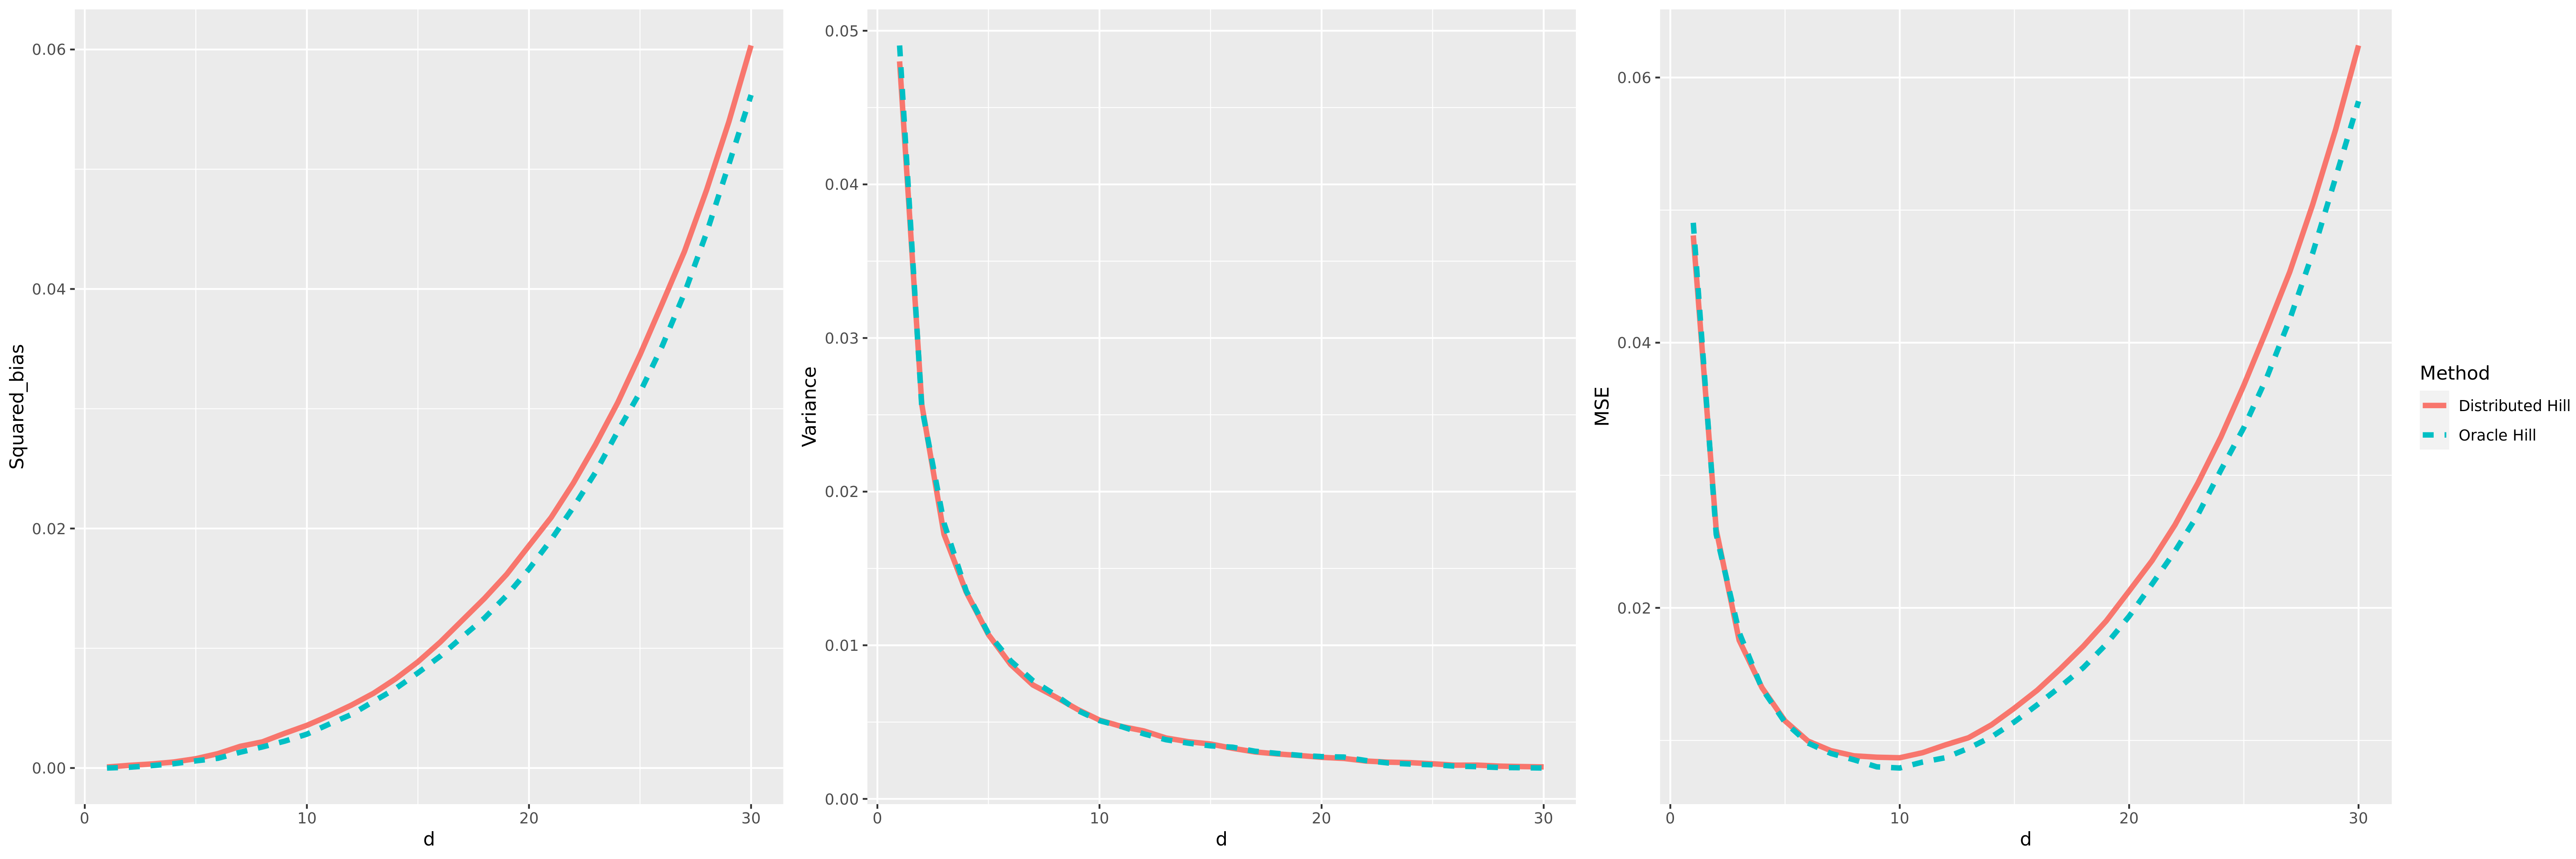
\includegraphics[width=0.65\textwidth]{Frechet_20_50_choice_d.png}
        }
        \subfigure[Pareto(1) Distribution]{
        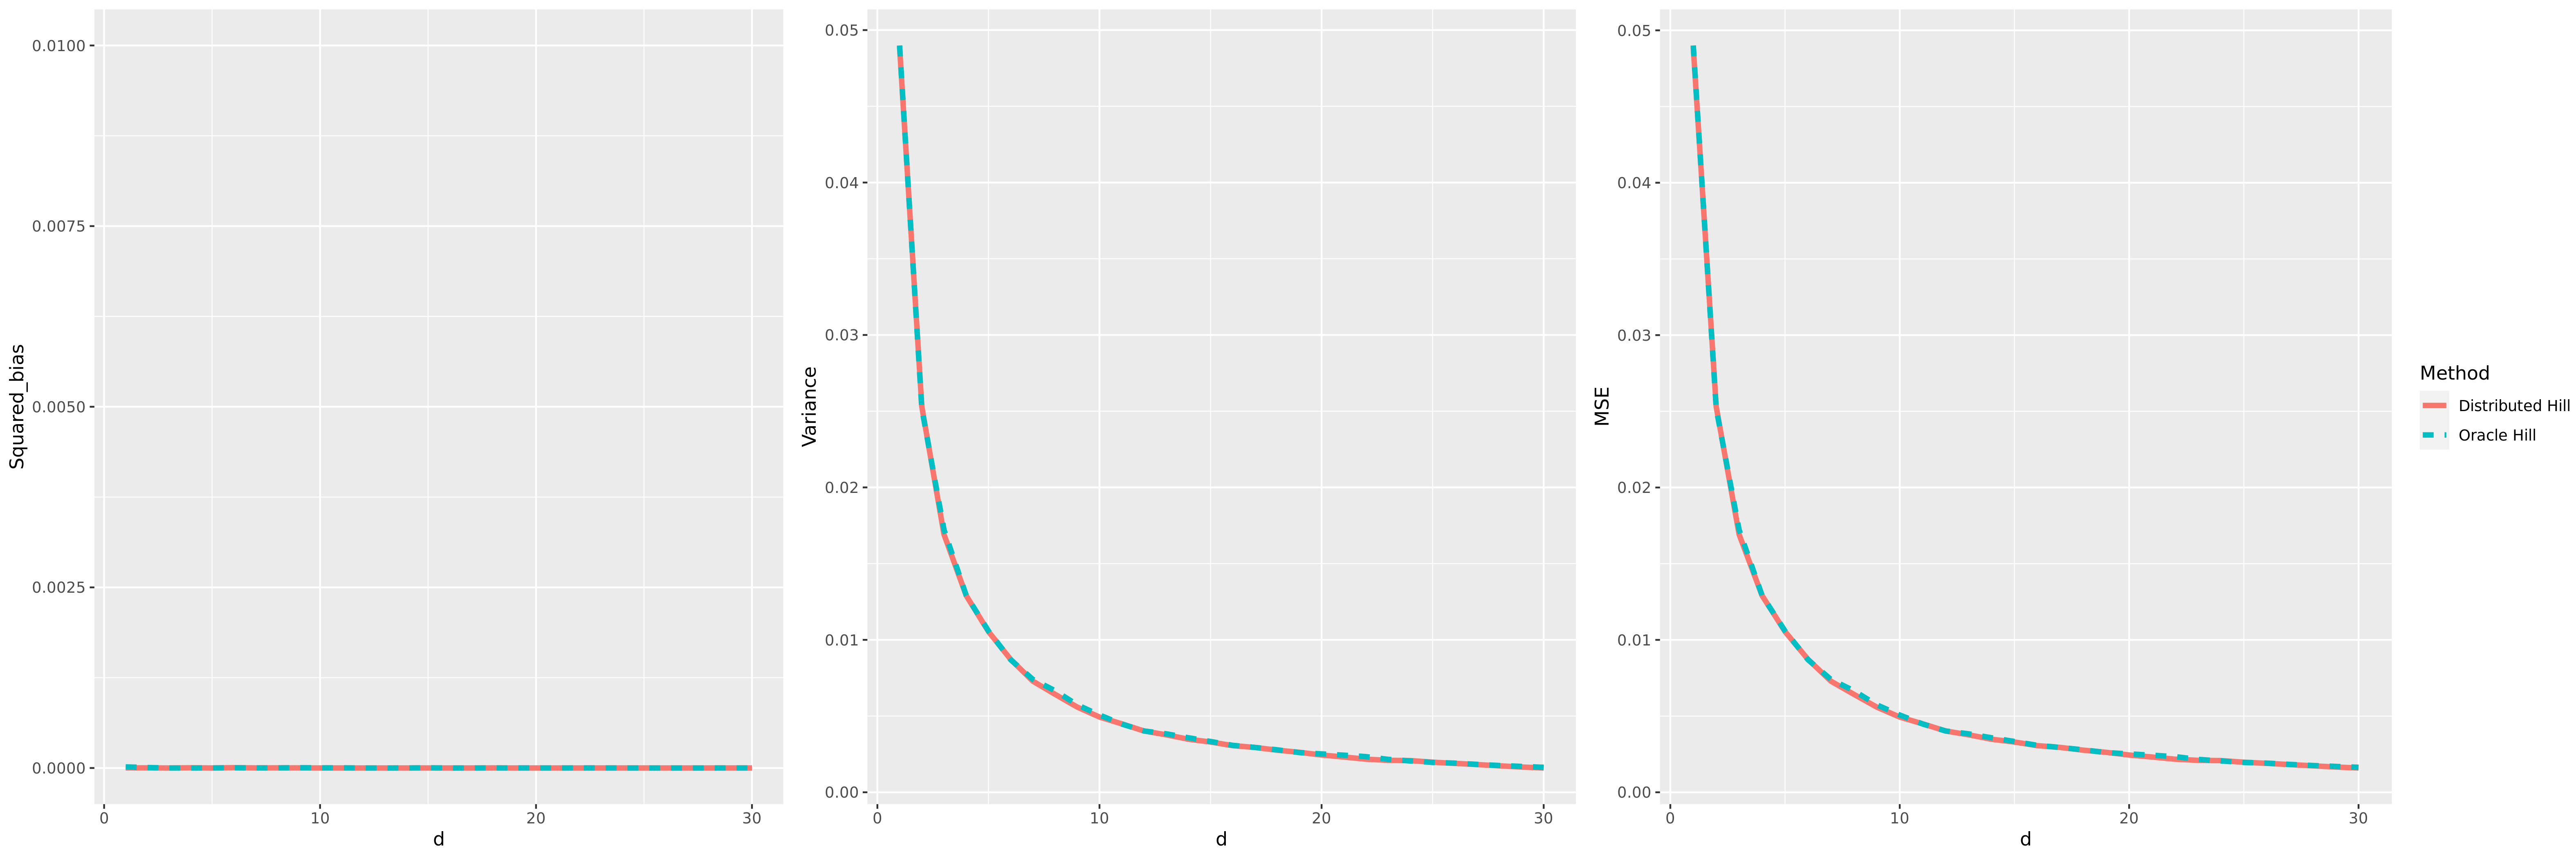
\includegraphics[width=0.65\textwidth]{Pareto_20_50_choice_d.png}
        }
    \end{figure}
\end{frame}

\begin{frame}
    \frametitle{Continue}
    \begin{figure}[htbp]
        \centering
        \subfigure[Absolute Distribution]{
        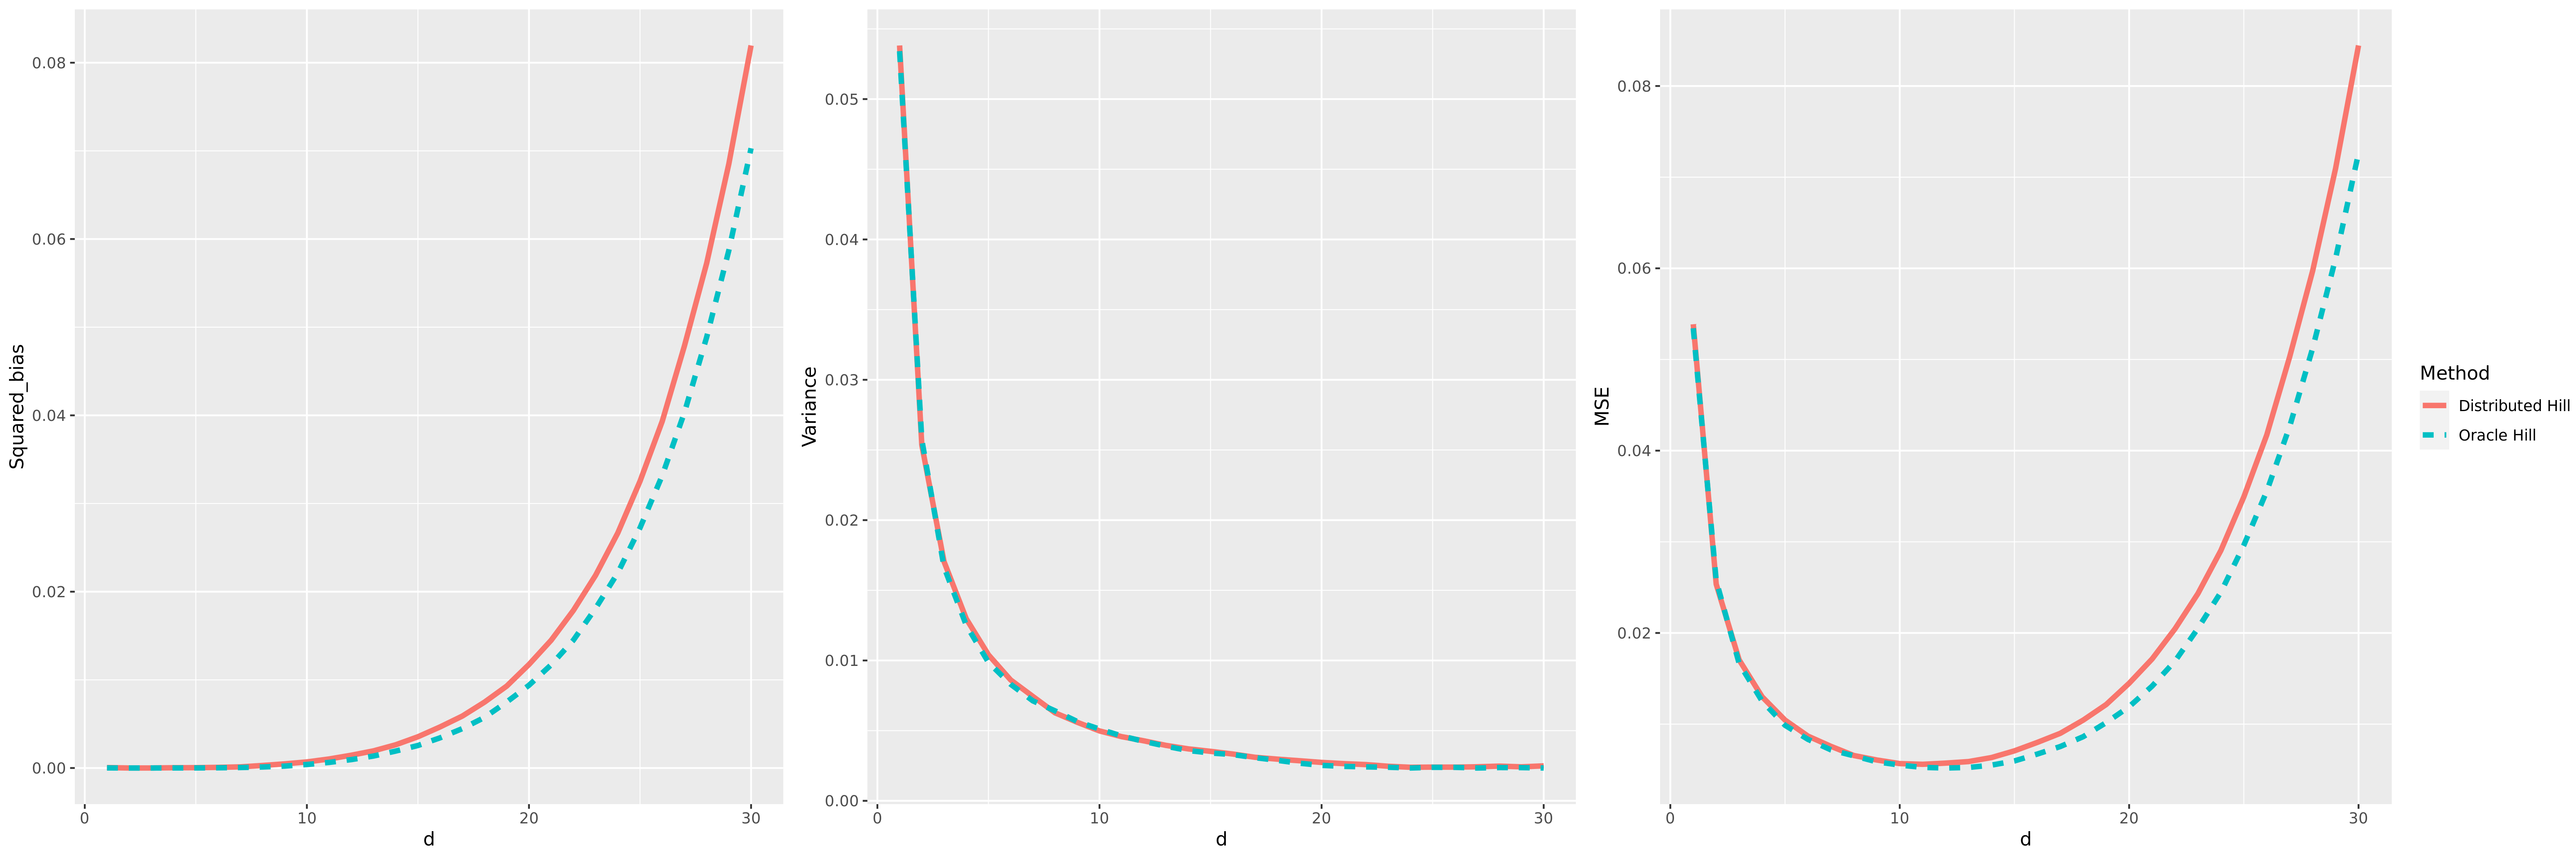
\includegraphics[width=0.65\textwidth]{Cauchy_20_50_choice_d.png}
        }
    \end{figure}
\end{frame}

\begin{frame}
    \frametitle{Simu2: Comparison for different level of $k$}
    Fix $d=2$ (a low level) and $d=8$ (an intermediate level.) The x-axis is the total number of exceedance ratios.
    \begin{figure}[htbp]
        \centering
        \subfigure[Fr\'echet(1) Distribution]{
        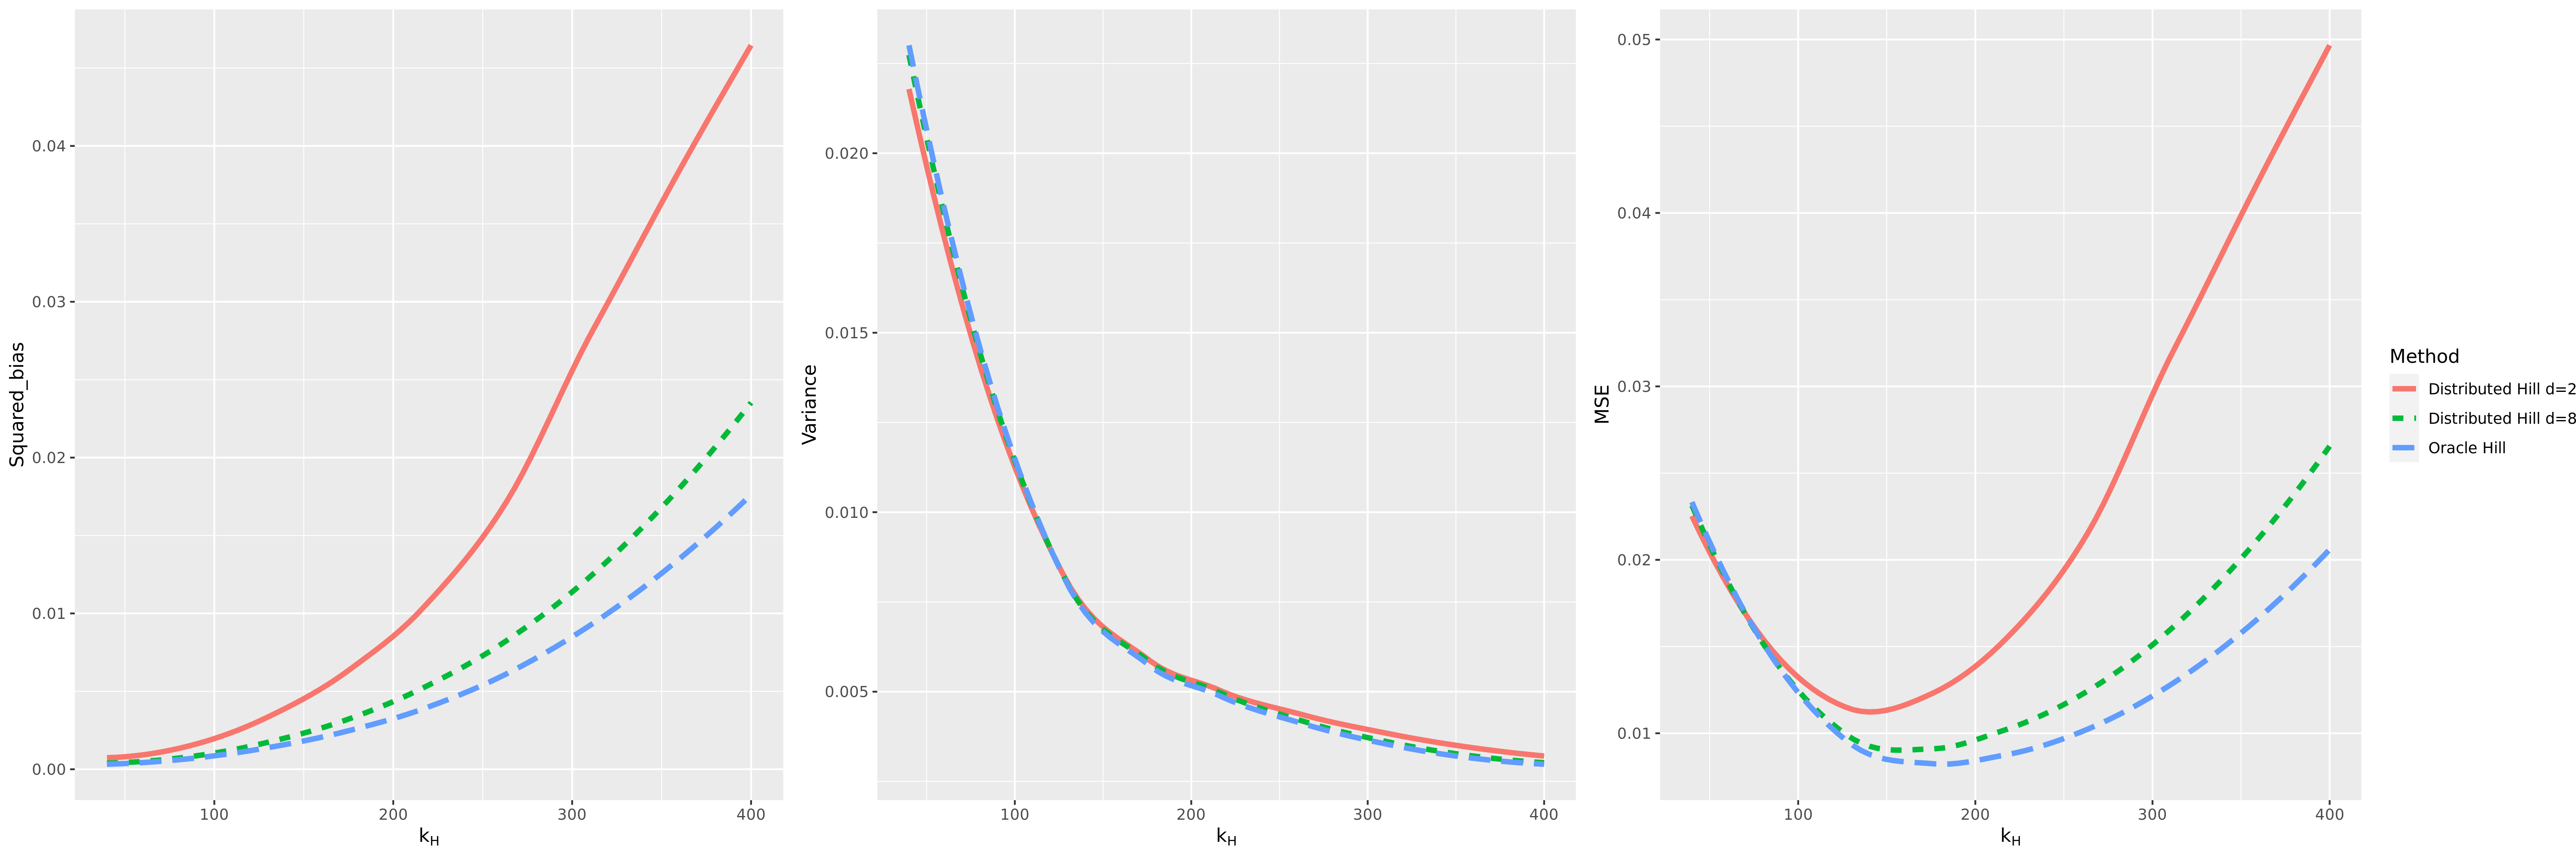
\includegraphics[width=0.65\textwidth]{Frechet_Oracle_1_kd.png}
        }
        \subfigure[Pareto(1) Distribution]{
        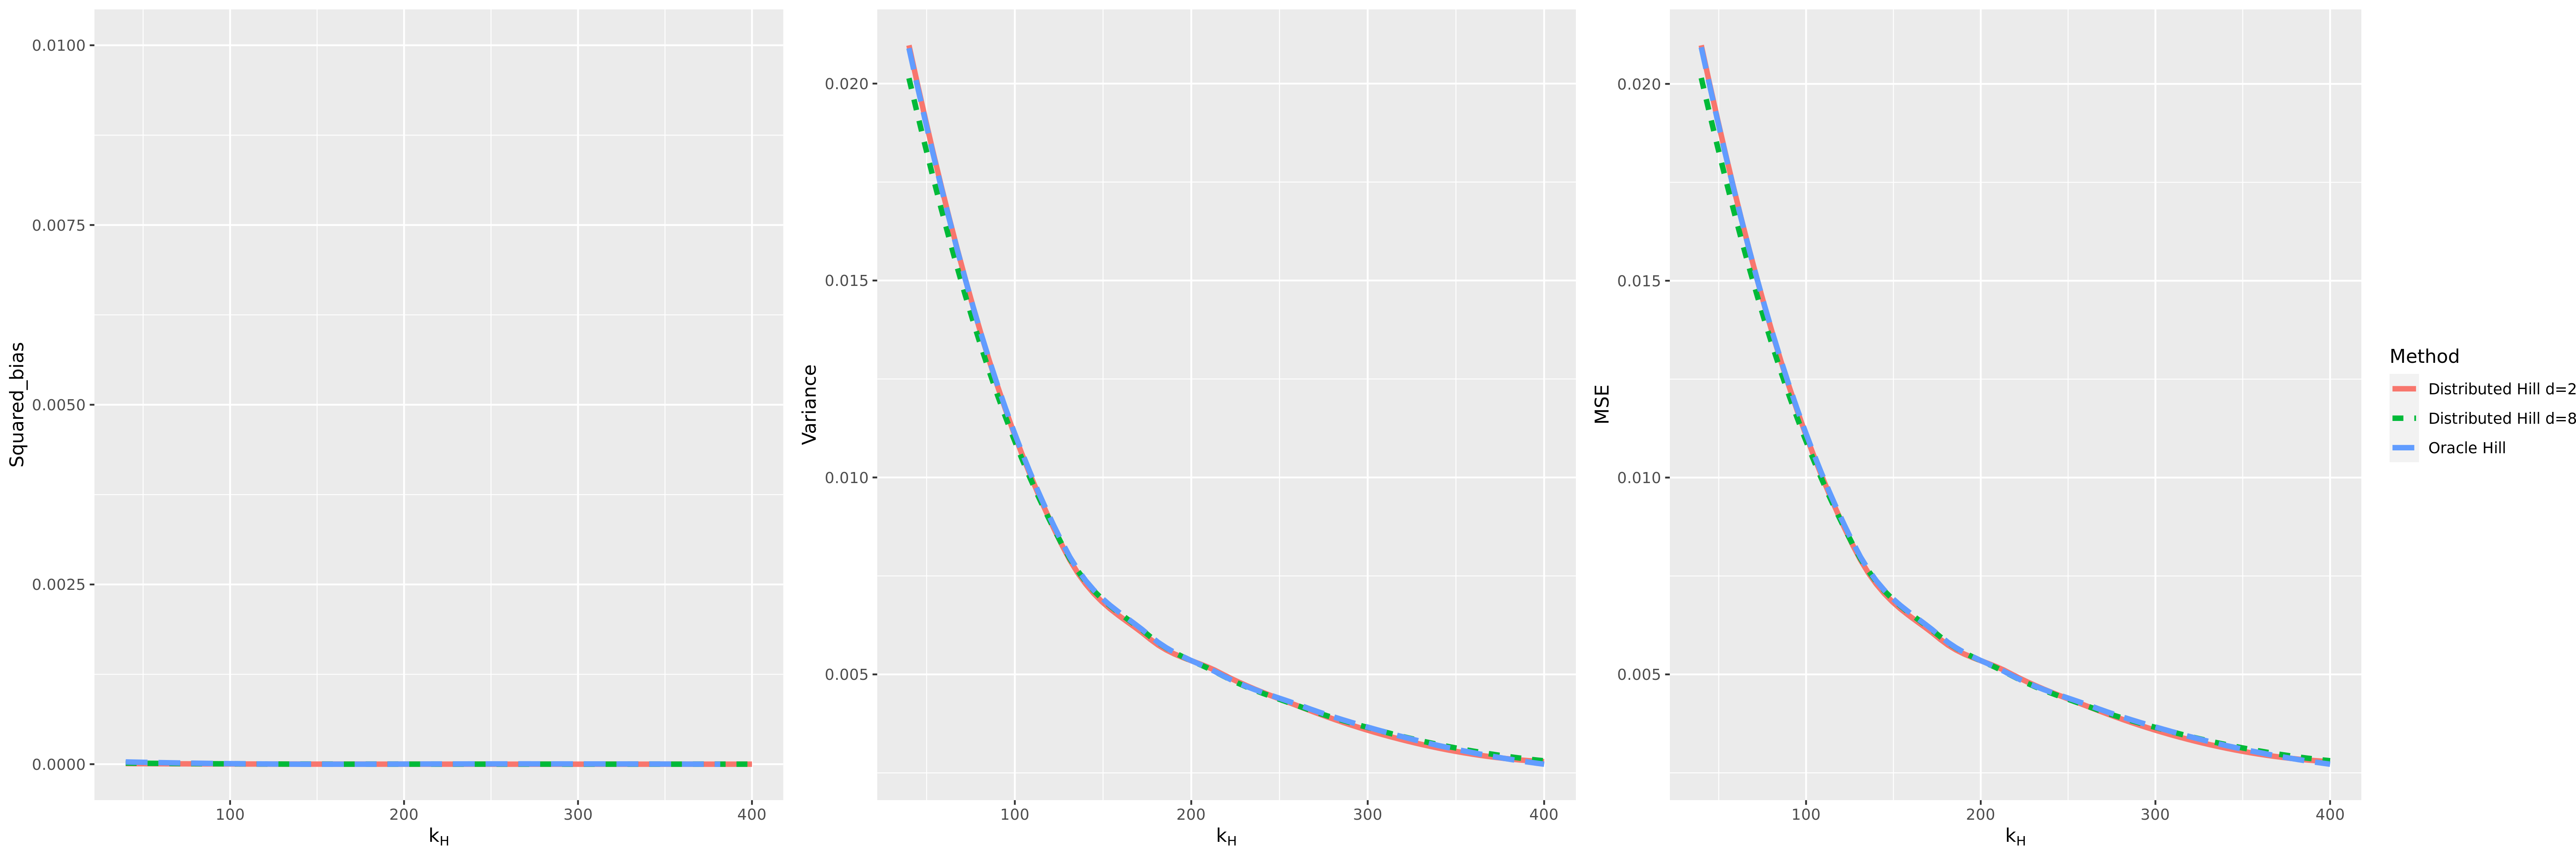
\includegraphics[width=0.65\textwidth]{Pareto_Oracle_1_kd.png}
        }

        \end{figure}
\end{frame}

\begin{frame}
    \frametitle{Continue}
    \begin{figure}[htbp]
        \centering
        \subfigure[Absolute Cauchy Distribution]{
        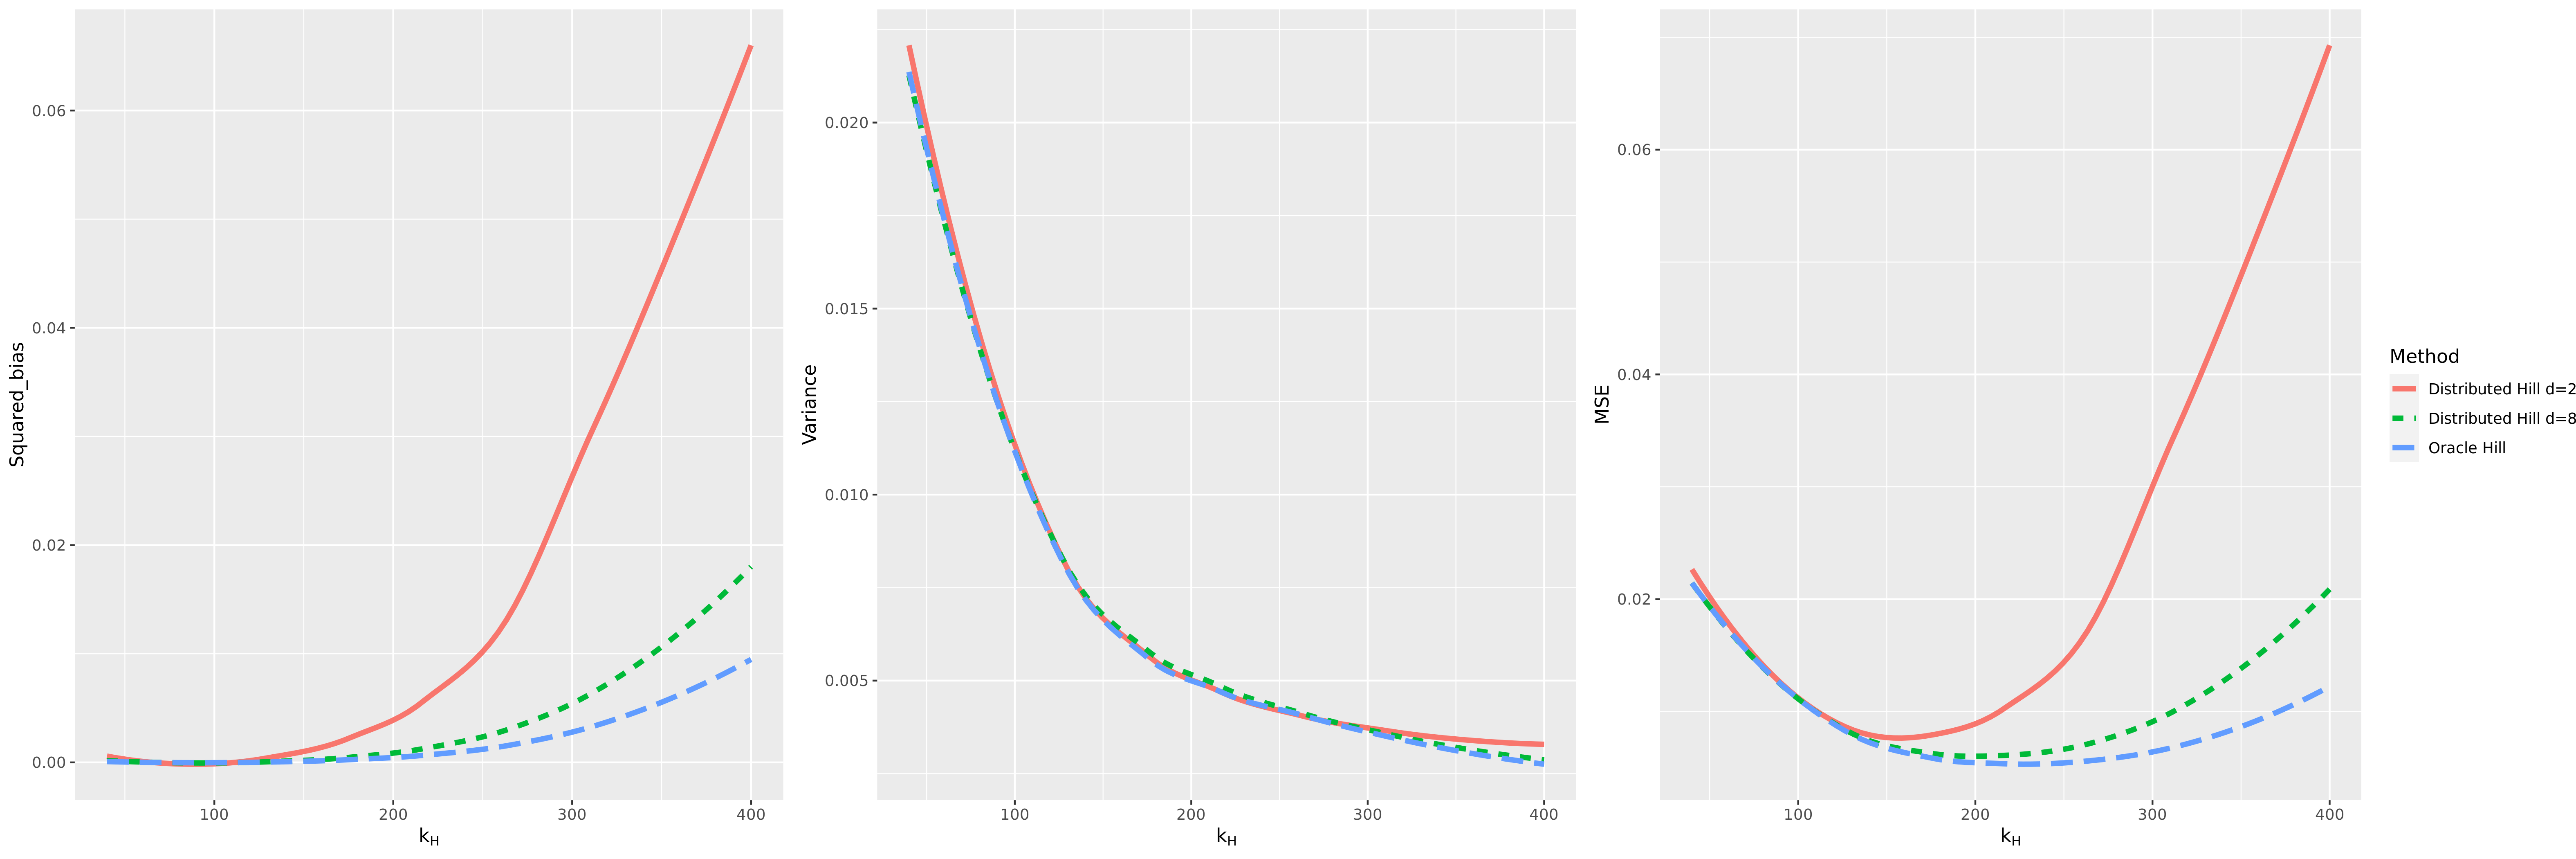
\includegraphics[width=0.8\textwidth]{Cauchy_Oracle_1_kd.png}
        }
        \end{figure}
\end{frame}

\begin{frame}
    \frametitle{Simu3: Comparison with block maxima MLE}
    \begin{figure}[htbp]
        \centering
        \subfigure[Fr\'echet(1) Distribution]{
        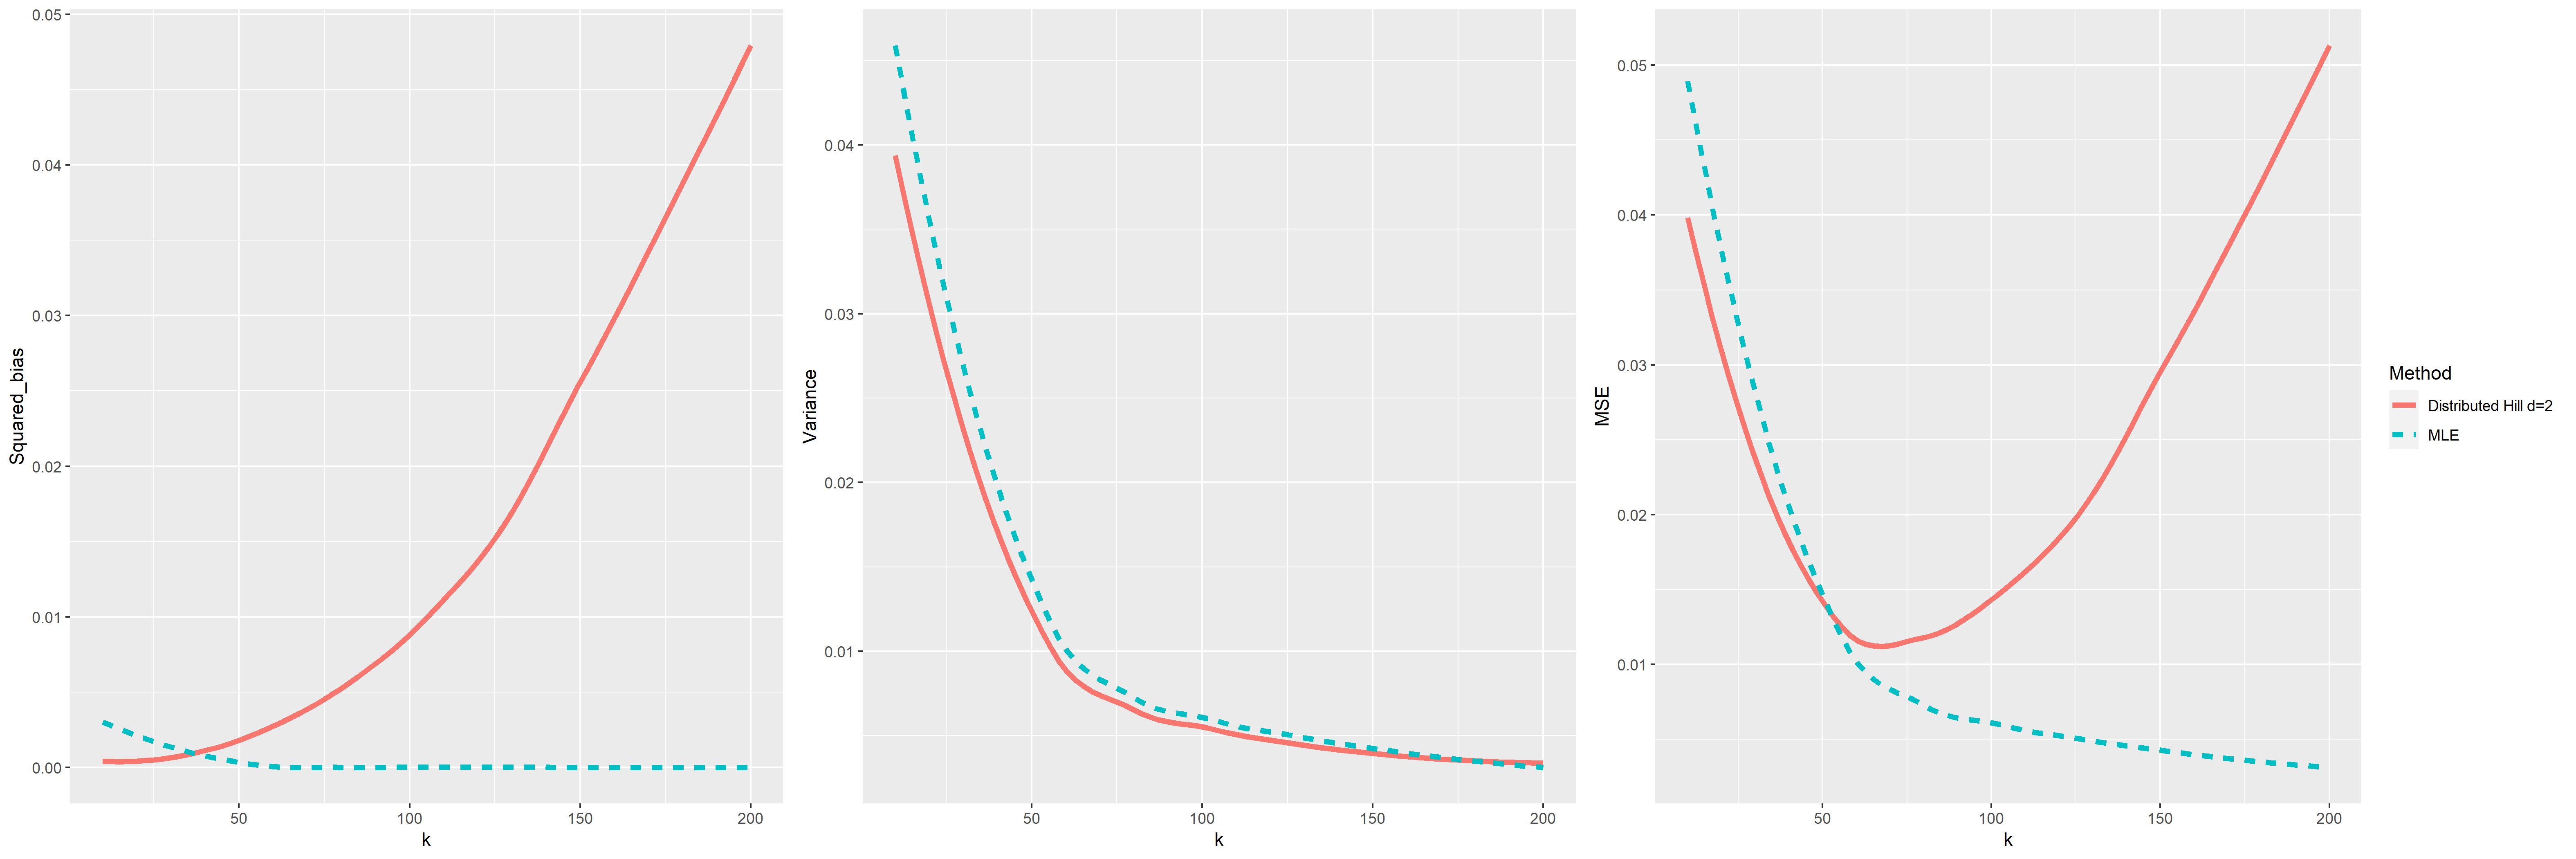
\includegraphics[width=0.7\textwidth]{Frechet_1_MLE.png}
        }
        \subfigure[Pareto(1) Distribution]{
        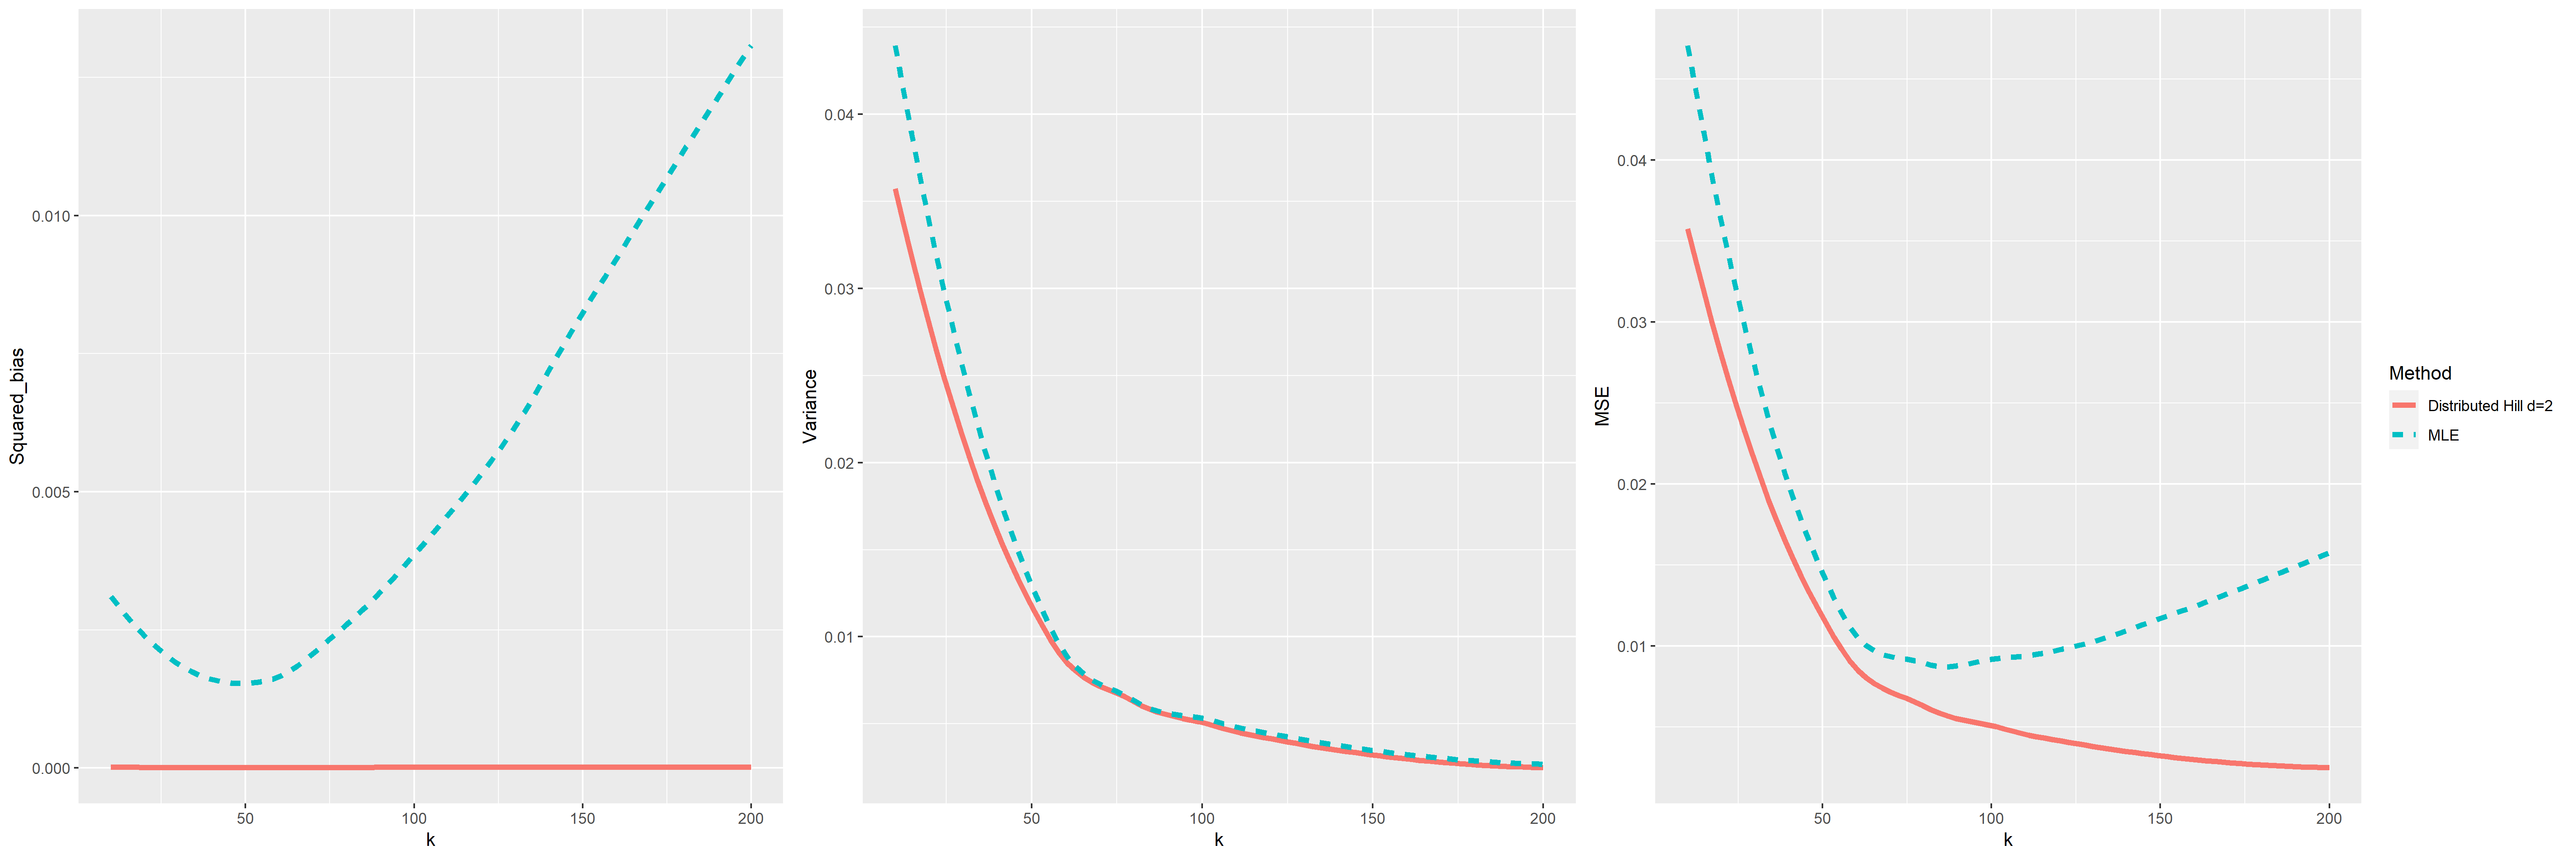
\includegraphics[width=0.7\textwidth]{Pareto_1_MLE.png}
        }
        \end{figure}

    

\end{frame}

\begin{frame}
    \frametitle{Continue}
    \begin{figure}[htbp]
        \centering
        \subfigure[Absolute Cauchy Distribution]{
        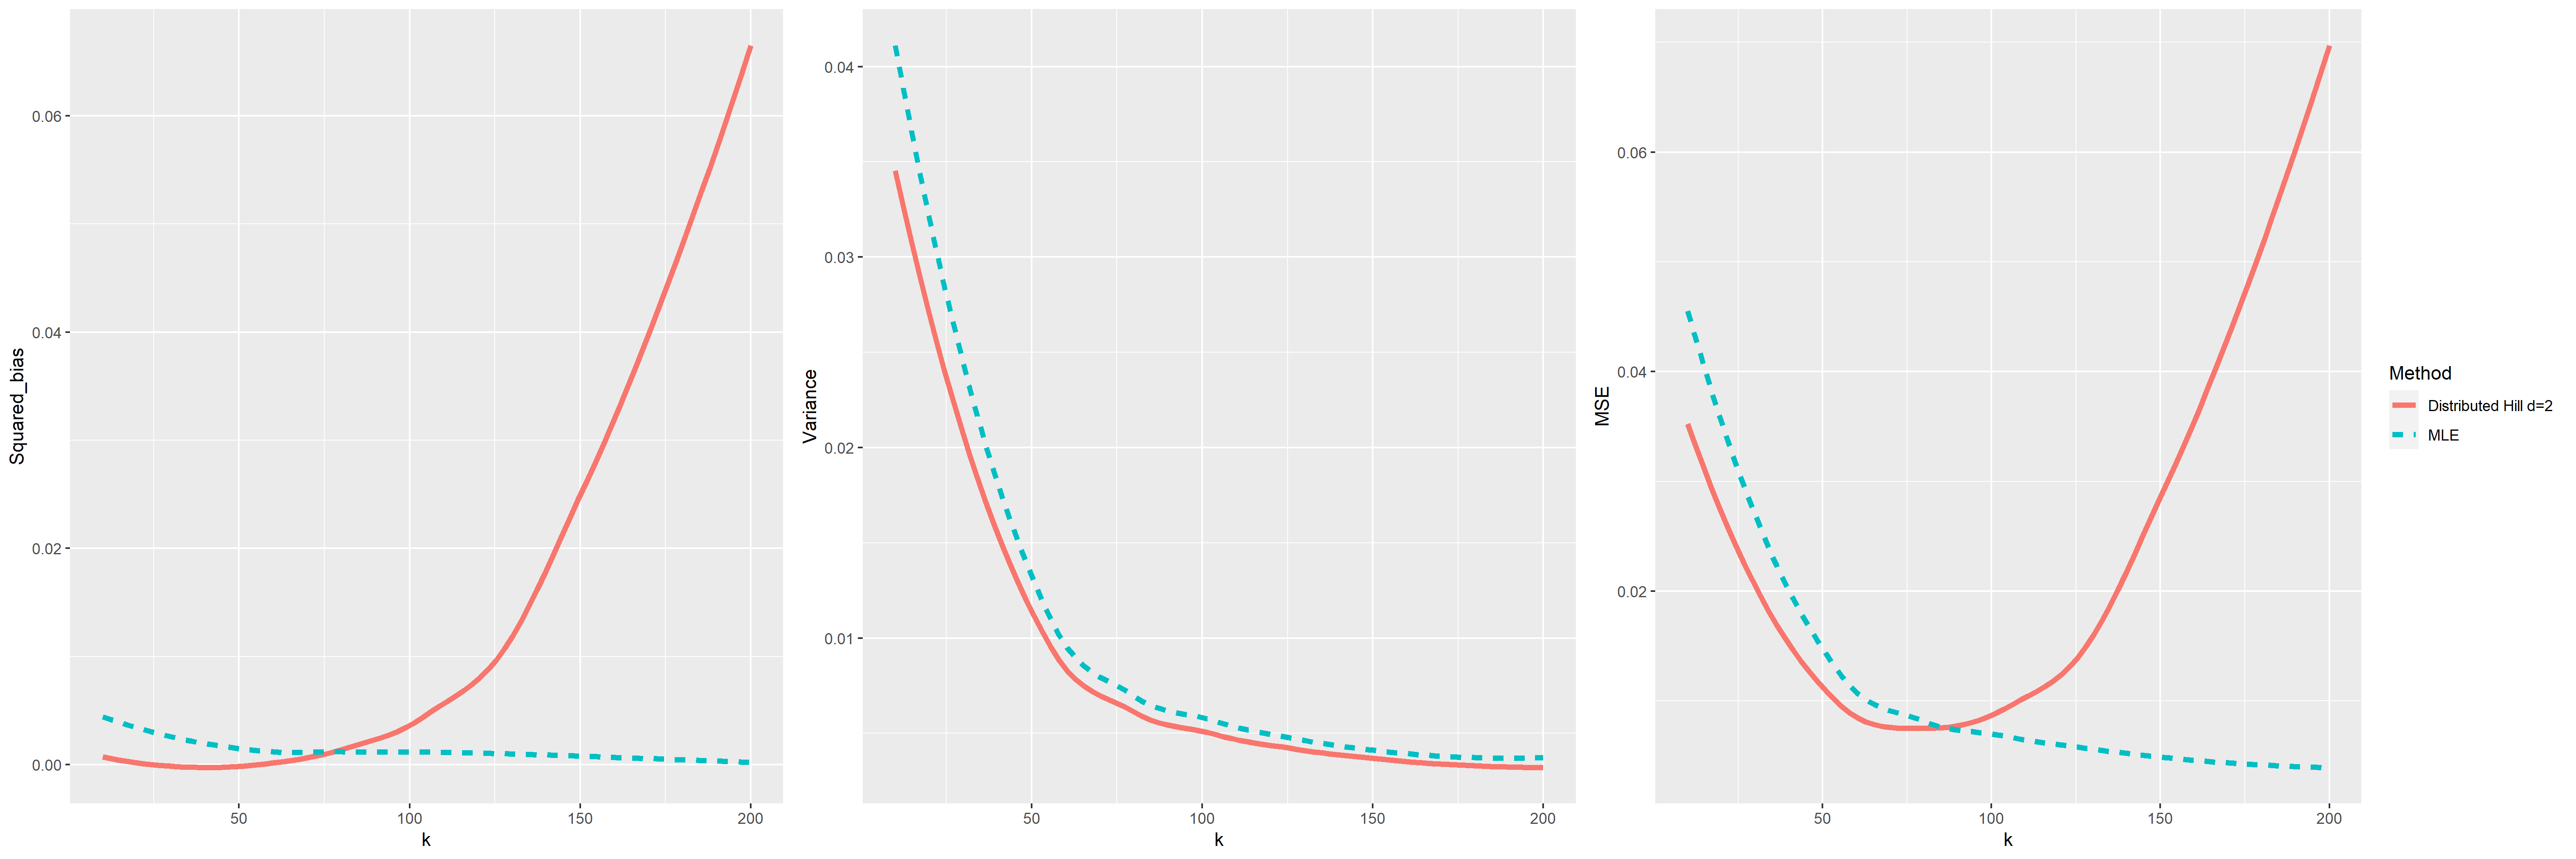
\includegraphics[width=0.8\textwidth]{Cauchy_1_MLE.png}
        }
        \end{figure}
    

\end{frame}
\section{Real Data Application}
\begin{frame}
    \frametitle{Dataset Description}
\begin{itemize}
    \item Car insurance claims in five states of the United States during January and February 2011.
    \bigskip
    \item We consider five hypothetical insurance companies, one in each state, where each company monopolies all the car insurance in its own state.
    \bigskip
    \item Due to business privacy, companies cannot share their data to others but they are willing to share their statistical results.
\end{itemize}
    

\end{frame}

\begin{frame}
    \frametitle{Dataset Description}
    The dataset contains 9134 observations, with 2601, 798, 3150, 1703 and 882 observations for Iowa,Kansas, Missouri, Nebraska and Oklahoma, repsectively. 
    \begin{figure}[htbp]
        \centering
          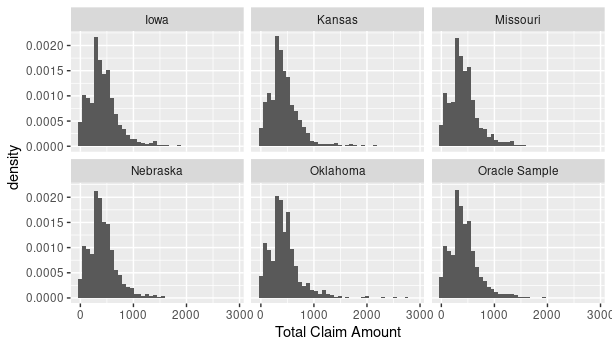
\includegraphics[width=0.8\textwidth]{histogram_full_data.png} 
      \end{figure}

\end{frame}

\begin{frame}
    \frametitle{}
    \begin{figure}[htbp]
        \centering
          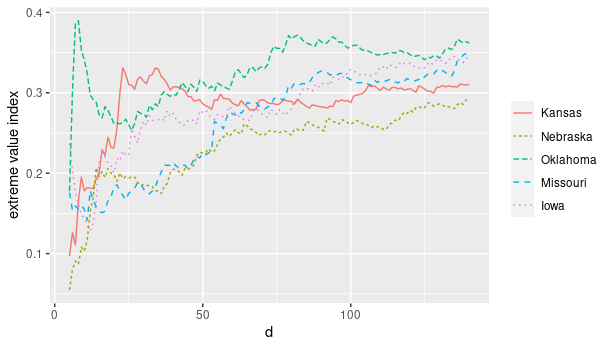
\includegraphics[width=0.8\textwidth]{gamma_state.png}
        \caption{Estimation for the extreme value index of total claim amount for each state.}
        \label{figure Insurance_example_gamma_state}
      \end{figure}
    
\end{frame}

\begin{frame}
    \frametitle{}
    \begin{figure}[htbp]
        \centering
          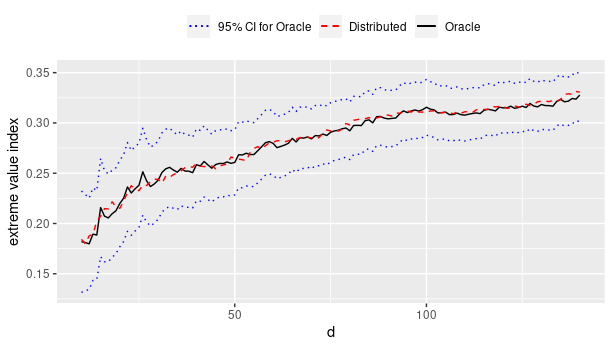
\includegraphics[width=0.8\textwidth]{DCvsOracle.png}
        \caption{The point estimation and the 95\% confidence interval of the distributed Hill estimator and the oracle Hill estimator for $\gamma$ of total claim amount. }
        \label{figure Insurance_example_gamma_DC}
      \end{figure}
    

\end{frame}
\end{document}
